%% bare_conf.tex
%% V1.2
%% 2002/11/18
%% by Michael Shell
%% mshell@ece.gatech.edu

% setup page to suit conference specification using fancyhdr
\documentclass[conference,letterpaper]{IEEEtran}

%\usepackage{fancyhdr}
%\setlength{\paperwidth}{215.9mm}
%\setlength{\hoffset}{-9.7mm}
%\setlength{\oddsidemargin}{0mm}
%\setlength{\textwidth}{184.3mm}
%\setlength{\columnsep}{6.3mm}
%\setlength{\marginparsep}{0mm}
%\setlength{\marginparwidth}{0mm}
%
%\setlength{\paperheight}{279.4mm}
%\setlength{\voffset}{-7.4mm}
%\setlength{\topmargin}{0mm}
%\setlength{\headheight}{0mm}
%\setlength{\headsep}{0mm}
%\setlength{\topskip}{0mm}
%\setlength{\textheight}{235.2mm}
%\setlength{\footskip}{12.4mm}

%\setlength{\parindent}{1pc}

\usepackage{lipsum}

\usepackage{fancyhdr}

% some very useful LaTeX packages include:

\usepackage{cite}
\usepackage{url}
\usepackage{amsmath}
\usepackage{stfloats}
\usepackage[section]{placeins}

\usepackage{graphicx}
\usepackage{epstopdf}


%\usepackage{subfigure} % Written by Steven Douglas Cochran
                        % This package makes it easy to put subfigures
                        % in your figures. i.e., "figure 1a and 1b"
                        % Docs are in "Using Imported Graphics in LaTeX2e"
                        % by Keith Reckdahl which also documents the graphicx
                        % package (see above). subfigure.sty is already
                        % installed on most LaTeX systems. The latest version
                        % and documentation can be obtained at:
                        % http://www.ctan.org/tex-archive/macros/latex/contrib/supported/subfigure/


% Other popular packages for formatting tables and equations include:

%\usepackage{array}
% Frank Mittelbach's and David Carlisle's array.sty which improves the
% LaTeX2e array and tabular environments to provide better appearances and
% additional user controls. array.sty is already installed on most systems.
% The latest version and documentation can be obtained at:
% http://www.ctan.org/tex-archive/macros/latex/required/tools/

% Mark Wooding's extremely powerful MDW tools, especially mdwmath.sty and
% mdwtab.sty which are used to format equations and tables, respectively.
% The MDWtools set is already installed on most LaTeX systems. The lastest
% version and documentation is available at:
% http://www.ctan.org/tex-archive/macros/latex/contrib/supported/mdwtools/


% V1.6 of IEEEtran contains the IEEEeqnarray family of commands that can
% be used to generate multiline equations as well as matrices, tables, etc.


% Also of notable interest:

% Scott Pakin's eqparbox package for creating (automatically sized) equal
% width boxes. Available:
% http://www.ctan.org/tex-archive/macros/latex/contrib/supported/eqparbox/


% Notes on hyperref:
% IEEEtran.cls attempts to be compliant with the hyperref package, written
% by Heiko Oberdiek and Sebastian Rahtz, which provides hyperlinks within
% a document as well as an index for PDF files (produced via pdflatex).
% However, it is a tad difficult to properly interface LaTeX classes and
% packages with this (necessarily) complex and invasive package. It is
% recommended that hyperref not be used for work that is to be submitted
% to the IEEE. Users who wish to use hyperref *must* ensure that their
% hyperref version is 6.72u or later *and* IEEEtran.cls is version 1.6b
% or later. The latest version of hyperref can be obtained at:
%
% http://www.ctan.org/tex-archive/macros/latex/contrib/supported/hyperref/
%
% Also, be aware that cite.sty (as of version 3.9, 11/2001) and hyperref.sty
% (as of version 6.72t, 2002/07/25) do not work optimally together.
% To mediate the differences between these two packages, IEEEtran.cls, as
% of v1.6b, predefines a command that fools hyperref into thinking that
% the natbib package is being used - causing it not to modify the existing
% citation commands, and allowing cite.sty to operate as normal. However,
% as a result, citation numbers will not be hyperlinked. Another side effect
% of this approach is that the natbib.sty package will not properly load
% under IEEEtran.cls. However, current versions of natbib are not capable
% of compressing and sorting citation numbers in IEEE's style - so this
% should not be an issue. If, for some strange reason, the user wants to
% load natbib.sty under IEEEtran.cls, the following code must be placed
% before natbib.sty can be loaded:
%
% \makeatletter
% \let\NAT@parse\undefined
% \makeatother
%
% Hyperref should be loaded differently depending on whether pdflatex
% or traditional latex is being used:
%
\ifx\pdfoutput\undefined
\usepackage[hidelinks,hypertex]{hyperref}
\else
\usepackage[pdftex,hidelinks,hypertexnames=false]{hyperref}
\fi


\begin{document}
% paper title
\title{A Path Planning Method Based on Genetic Algorithms and Curve Fitting Techniques}
\newcommand{\Keywords}{Genertic Algorithms, Curve Fitting, Path Planning, Grid Method, Robotics}

% author names and affiliations
% use a multiple column layout for up to three different
% affiliations
\author{
\IEEEauthorblockN{Brock Kopp}
\IEEEauthorblockA{Mechatronics Engineering\\
	University of Waterloo\\
	Waterloo, Ontario\\
	brock.kopp@uwaterloo.ca}
\and
\IEEEauthorblockN{Karl Price}
\IEEEauthorblockA{Mechatronics Engineering\\
	University of Waterloo\\
	Waterloo, Ontario\\
	karldprice@gmail.com}
\and
\IEEEauthorblockN{Angelica Ruszkowski}
\IEEEauthorblockA{Mechatronics Engineering\\
	University of Waterloo\\
	Waterloo, Ontario\\
	aruszkow@uwaterloo.ca}}

% make the title area
\maketitle
\thispagestyle{plain}

% insert page header and footer here for IEEE PDF Compliant
\fancypagestyle{plain}{
\fancyhf{}	% clear all header and footer fields
\fancyfoot[L]{}
\fancyfoot[C]{}
\fancyfoot[R]{}
\renewcommand{\headrulewidth}{0pt}
\renewcommand{\footrulewidth}{0pt}
}

\pagestyle{fancy}{
\fancyhf{}
\fancyfoot[R]{}}
\renewcommand{\headrulewidth}{0pt}
\renewcommand{\footrulewidth}{0pt}


\begin{abstract}
% CRITERIA	(4 Senetences)
	% ?1. State the problem
	% ?2. Say why it�s an interesting problem
	% ?3. Say what your solution achieves
	% ?4. Say what follows from your solution
%
Navigation and path planning are critical components of developing robotic technology, where optimized path planning can improve efficiency and throughput of an industrial robotic manipulator. A genetic algorithm is used to plan a polynomial function based trajectory which avoids collisions with any obstacles and minimizes path distance and dynamic constraints. The stochastic nature of the genetic algorithm allows it to determine a viable and efficient path for a manipulator quickly as its environment changes. Algorithm results are verified by comparing with deterministic algorithms which produce the absolute best path.
\end{abstract}

\vspace{3mm}	%Brock

\begin{IEEEkeywords}
\Keywords
\end{IEEEkeywords}

\section{Introduction} \label{sec:introduction}
% CRITERIA	(1 Page)
	% 1.Describe the problem
	 % - Use Examples
	 % - Present the general case
	% 2.State your contributions
		% -Present a list of contributions
Path planning is a critical component of navigation technology, and a fundamental area in robotics research. Verifying path safety is critical for both the welfare of the robot as well as its surrounding environment, which can contain people or valuable infrastructure. The path must ultimately reach its destination while satisfying specified criteria, the most common of which is distance (or time). Another important criterion is path dynamics, where the forces and other dynamic characteristics of the robot are considered. Excessive acceleration and jerk cause stress on the robotic manipulator and degrade robot tracking characteristics, which are often a function of acceleration. These criteria are accounted for by relatively few common path planning algorithms \cite{elshamli04}.

Path planning techniques can be applied to industrial robotic manipulators to ensure efficient operation while maneuvering safely in the environment. Articulated manipulators are bounded to their configuration workspace, which is a two-dimensional representation of their allowable motion range \cite{kavraki96}. Frequently used algorithms for motion planning include probabilistic road maps, potential field methods, and neural network approaches \cite{sharir89,khosla88,rimon92,yang00}. Since every robot has a unique and complex task and environment, a robust solution is necessary. Genetic algorithms are especially suited for such complex optimization problems \cite{renner03}.

As a stochastic optimization technique, it is expected that a genetic algorithm will find the global optimum for a problem in a reasonable amount of time and computational cost. Due to the iterative evolutionary nature of genetic algorithms however, computational time may still be greater than other probabilistic algorithms. Overarching these concerns, the robustness of the genetic algorithm, combined with its ability to easily evaluate all path criteria of the optimization problem make it an appealing solution.

The robot's environment and obstacles will be represented in a discretized grid, and polynomial curve fitting techniques will be used to define the optimum path from the start to the end location through the specified environment. The curve fitting method helps simplify and expedite the generation of a desired path, compared to commonly used techniques such as rapidly exploring random trees \cite{rodriguez06}. The genetic algorithm will determine the polynomial coefficients which result in a curve with the greatest fitness, as determined by the constraints of the problem (namely path distance and jerk). A polynomial function was selected to describe the path since it inherently results in a continuous trajectory rather than traditional discontinuous way point based trajectories.

While there is no absolute best path planning algorithm for all situations, it is proposed that:

\begin{itemize}
	\item A Genetic Algorithm can effectively plan a path through a robotic manipulator's configuration space, producing a valid result 94\% of the time.
	\item The algorithm presented can plan a path which not only minimizes distance traveled, but also accounts for robotic manipulator dynamics such as acceleration and jerk.
	\item The algorithm can identify a viable solution which is within 1\% of the shortest distance as determined using a deterministic algorithm such as wavefront, while showing improvements to computation time.
\end{itemize}


\section{Background Review} \label{sec:background}
% CRITERIA	(1 page)
	% ?Materials & Method
	% ?Datasets
	% ?Materials (sources)
	% ?Methods (reference and brief description)
	% ?Proposed approach: algorithm
	% ?Equations and formulas
%
Path planning is an active area of research due to the complexity of the problem and the need for a robust solution applicable to various environments. Many algorithms exist, but none of the proposed algorithms are capable of encompassing all the problem constraints for all environments \cite{sariff06}.

Existing path planning solutions include reactive motion planning algorithms, graph and probabilistic based motion planning, and optimization based planning \cite{waslanderI}. Each of these has advantages and disadvantages with regards to planning a route through a robot's environment. Reactive planning algorithms such as potential field and wavefront methods are simple in concept however these are local approach methods and do not consider dynamic constraints. Some are inherently susceptible to local minima, making them unacceptable for obstacle avoidance \cite{koren91}. 

The wavefront method is designed to find the absolute shortest path, and as such will be used as the benchmark against which results from the suggested algorithm will be measured. It is expected that while the suggested algorithm will generate a longer path, the dynamic constraints will be satisfied, unlike the results of the wavefront solution.

Graph based planning offers a global approach. Graphs may be generated both deterministically (visibility graphs, cell decomposition, Voronoi diagrams), or randomly (probabilistic road maps). Established algorithms (such as Dijkstra's shortest path search) are used to extract the shortest path from the graph \cite{dijkstra59}. However dynamics of the robot are ignored in the generation of the graph, and this is detrimental to the criterion of path smoothness. Challenges also arise when there are restrictive obstacles such as narrow passages, however research in areas such as probabilistic road maps (PRMs) offers promising solutions \cite{hsu03}. Optimization based planning offers more confidence in finding a global optimum, however it is hindered by a lack of robustness: a poorly formulated problem may never converge \cite{waslanderIII}. It is also difficult to define obstacles.

In an effort to provide a simple method of avoiding obstacles and defining a path, the manipulator's configuration space will be discretized using a grid-based approach, and curve fitting techniques will be employed to find the ideal path. The configuration space of a robotic manipulator is a transformation of the manipulator's joint space to a two-dimensional Cartesian space. Defining the environment with a grid-graph may not be the most effective (cell decomposition offers greater efficiency \cite{lingelbach04}), however it provides a simple way to define obstacles as well as flexibility in representation. The grid will represent the configuration space for an articulated industrial robot. The grid cell size will define the computational resources required. A trade-off between resolution in the grid and computational efficiency must be made.

B\'{e}zier curves have been suggested to define the fitted curves generated by the genetic algorithm \cite{choi10}. B\'{e}zier curves provide smooth paths between two vectors, and while very effective for lower-dimensional problems, B\'{e}zier functions become very computationally expensive as the problem dimensionality increases. This paper therefore aims to use polynomial curve fitting in combination with genetic algorithms to optimize the curve. The curve will be optimized by minimizing distance, maximizing smoothness (minimizing jerk), and ensuring a safe passage around all obstacles. Genetic algorithms present an appealing approach for such complex optimization problems and offer good robustness as well \cite{zou12}.

The father of genetic algorithms, John Holland, modeled this machine intelligence technique after Darwin's Theory of Evolution, and the concept of ``survival of the fittest'' which he observed in nature. There are two natural learning epitomes available: the brain and evolution. Holland was inspired by the fact that the processes of natural evolution and natural genetics have become elucidated over decades of study in biology and molecular biology \cite{goldberg88}. The subtleties of the fundamental mechanisms of the brain, in contrast, are still shrouded in mystery. As such it seems clear to use the better understood model of genetic evolution as a platform for an optimization technique.

Research has already been done regarding the application of the parallel heuristic search method of genetic algorithms to curve fitting \cite{gulsen95,karr91,ismail08}. This paper builds upon that research. The goal is to find the coefficients of a polynomial function that will define a path with optimized path criteria. Thus each chromosome will contain a set of function parameters, labeled $\{P_3, \ldots, P_0\}$ in Equation \ref{eq:polyTraj}.

\begin{align} \label{eq:polyTraj}
	\phi = P_3*\theta^3 + P_2*\theta^2 + P_1*\theta + P_0
\end{align}

Testing will be performed by creating random environments containing arbitrarily place objects. The algorithm will then plot a trajectory between a randomly defined start and end point. Many iterations of these tests will be performed in a variety of environments in order to accurately determine the effectiveness of this algorithm. The average path distance for each environment will be compared to the minimum distance as calculated by a Wavefront algorithm \cite{waslanderI}.

The wavefront algorithm is a deterministic algorithm which is capable of finding the shortest path between two points through a discretized environment. This will provide a ``gold standard'' which can be used to evaluate the performance of the genetic algorithm. Since the genetic algorithm is a stochastic search, it will not result in an identical path twice. As such all results will be presented as averages and their associated distributions.

The result will be a global path planning algorithm functional in a static environment. Dynamic environments are possible with the proposed algorithm, however computational efficiency must be optimized in order to minimize the time required to find the solution. This new application offers a simple way to determine a path while taking into consideration all the defined path criteria.


\section{Method} \label{sec:method}
% CRITERIA	(2-3 pages)
	% -Check that each claim in the intro is addressed
	% -Forward reference evidence from a claim
	% -Present the experiments
	% -Analyze raw data
	
% OUTLINE
	% - Setup
		% - Criteria (Fitness)
			% - Distance (low weight since it doesn't really matter)
			% - Obstacle avoidance (Hight weight, mission critical)
			% - Minimize jerk (Mid weight)
		
		% - Touch breifly on encoding
			% - High order polynomial
			% - Chromozome - integer encoding
		% - Reporduction
			% - Random crossovers
		% - Mutation
			% - Defaults or Gusen's?
			% - Which worked out, why didn't the other?
		% - Initialization
			% - Random, pop size
		% - Termination
			% - Diversity convergence
			% - Or top half not coliding.
			% - Which worked out, why didn't the other?
			
		
	% - run with randomly generated environments (or at least 
		% - 1-5 objects
		% - placed randomly w/o overlap
		% - varying but constrained size
		% - fized start/end points
		% - Run 1000 times
		% - analyze data
		% - store data (map and the resultant path)

The Genetic Algorithm (GA) formed the basis for the experiemnts. Significant effort was expended setting up the GA in advance of testing, since without a well structured algorithm, the testing was sure to show poor results. The GA was implemented on Matlab, using the built-in GA libraries in order to avoid unnecessary development. While the base functionality was used, there remained many design considerations.

\subsection{Criteria}

\subsection{Configuration Space}
Commanding a robotic manipulator's position is complicated by the fact that it cannot be specified is X-Y-Z coordinates, but rather must be commanded using joint angles. Not only is this not intuitive for a human, but existing planning techniques function using more standard X-Y or X-Y-Z coordinate systems. As such, the robot's workspace was converted into a Configuration Space. Figure \ref{fig:ws2cs} shows both the workspace and the configuration space for a 2-DOF robot in an arbitrary workspace. The robotic manipulator's two degrees of freedom are denoted by the blue and red lines (each DOF respectively). The alloable robot configurations denoted in the Configuration Space by whitespace, while collisions are denoted by black.

\begin{figure}[h]
	\centering
	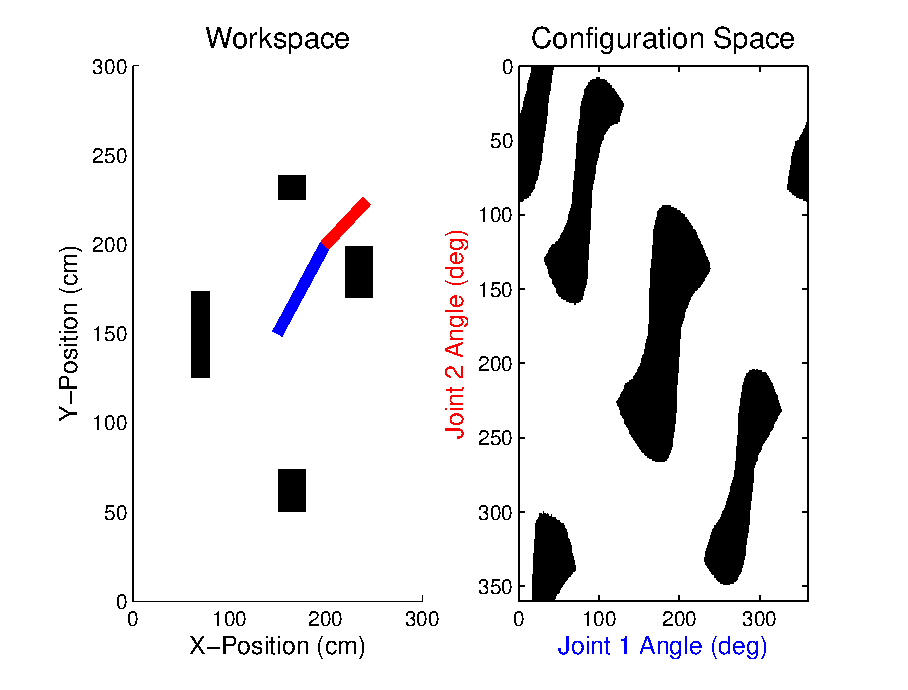
\includegraphics[width=3.5in]{./figures/wp2cs.eps}
	\caption{Conversion from robot workspace to configuration space }
	\label{fig:ws2cs}
\end{figure}

In the configuration space, robot tracjectories can be easily identified by either a human or a motion planning algorithm. This angle-angle plot can then be used to implement a polynomial trajectory, of which optimal coefficients can easily be solved using a Genetic Algorithm. The parameterized trajectory is denoted in Equation \ref{eq:polyTraj}.

\begin{align} \label{eq:polyTraj}
	\phi = P_4*\theta^4 + P_3*\theta^3 + P_2*\theta^2 + P_1*\theta + P_0
\end{align}

\subsection{Encoding}
The GA was developed using a linear encoding scheme, where a chromosome was defined to be an array of the polynomial function's coefficients (denoted as $\{P_0, \ldots, P_4\}$ in Equation \ref{eq:polyTraj}). Therefore, the GA would ultimately return the ideal set of coefficients for a function which would describe the optimal path for the robotic manipulator. These coefficients were limited to a range of [-50,50], since larger coefficients guarantee an invalid path since it would be too large and leave the workspace. While larger coefficients do not adversely affect the result of the algorithm, the increased diversity requires significantly larger computational resources which were not avaliable.

\subsection{Reproduction and Mutation}
/

\subsection{Initialization and Termination}



\textbf{SECTION REQUIREMENTS}
\begin{itemize}
\item Check that each claim in the intro is addressed
\item Forward reference evidence from a claim
\item Present the experiments
\item Analyze raw data
\end{itemize}

\section{Results} \label{sec:results}
% CRITERIA	(2-3 Pages)
	% -Stats & Distributions

% OUTLINE
	% - Distance of ours compared to the wavefront
	% - Dynamics, how often they are under an acceptable value
	% - How many times it finds a sucessful path w/o collisions
	% - Calculation time compared to wavefront
	
\subsection{Results}



\section{Discussion} \label{sec:discussion}
% CRITERIA (Half a page)
	% - Main findigs
	% - What results mean
	% - Limitations of our method
	% - Comparison of our results (Campare to probabilistic path planning)
	% - Need for further studies
	
% OUTLINE
% - Main findings
	% - Worse distance than wavefront *complete (could use more info?)
	% - Expect success in reducing jerk *complete
		% - Find a metric
		% - Find a gold standard
	% - 100% success of finding a path w/o collisions
	% - Slower than wavefront *complete
	% - num generation *complete
<<<<<<< HEAD
=======

>>>>>>> bcb99cb940c889ffd72195bbb00ac80b39f7c886
%% Length
Evaluating the performance of the genetical algorithm (GA) was complicated by its ability to consider many factors when determining the best path. These factors included path distance, vehicle dynamics and most importantly, obstacle avoidance. In order to determine a profile of the GA's performance, 600 tests were completed over the 15 random point configurations in 3 different environments.

The length of the path generated by the GA approach was on average 0.7\% longer than the path generated by the wavefront method to which it was compared. The wavefront is a deterministic environment which will find a very short path around obstacles, with no consideration for vehicle dynamics. The GA works differently in that it is a stochastic algorithm that is sampling the environment in an effort to find the shortest path. As such, it can get stuck in a local minimum and not ultimately return the path of best fitness. While processes internal to the GA attempt to avoid these situations, it is not a perfect algorithm.

The GA was able to determine a shorter path than the wavefront algorithm 474 of 600 (79\%) independent tests, despite attempting to also minimize jerk (sometimes at the cost of a longer path). While the GA is able to find a shorter path around obstacles 79\% of the time, it is still on average 0.7\% longer than wavefront since occasionally it will have an extrememly long path. These long paths are a result of the GA finding a local minimum and getting stuck there. In an actual implementation, the GA could be run multiple times in an effort to filter out local minima.

%% Speed
The GA was found to be much quicker at finding a solution than the wavefront algorithm. The wavefront algorithm took an average of 17 minutes and 50 seconds to analyze the shortest path between two points on any of the three test spaces used in this study. In comparison, the genetic algorithm took an average of 5.15 seconds to find the optimal path (20767\% improvement). While the actual algorithm execution time is abitrary and based on algorithm implementation, three orders of magnitude faster shows that the GA is conclusively faster than the wavefront algorithm. With execution times in the seconds, it is not unfathomable that this algorithm could be implemented live on a robotic manipulator who's environment was liable to change infrequently.

The algorithm was found to convege to a solution on average within 12.3 generations, with a standard deviation of 2.58 generations. This represents a fast convergence of the algorithm to a single solution.

%% Collisions
If was expected to be able to develop an algorithm that would find a valid path which never collided with an obstacle. The results from the experiment show that the algorithm infact finds a collision-free path 565 times in 600 (94\%) of the time. While this was not the anticipated result, it still constitutes a valid solution to the problem. In an industry application, if the algorithm produces a path which collides with an obstacle, it would simply re-initialize polulation. With a run time of 5.15 seconds, restarting the algorithm would not be prohibitive for most applications.

%% Jerk
Since trajectories varied between environments and start/end location, a reference jerk could not be identified. The jerk of a path was therefore compared to another instance of the GA where jerk was excluded from the fitness function. This allowed the effect of the jerk reduction to be quantified against a reference given a constant environment. It was found that the algorithm reduced path jerk by an average of 192\%. Ultimately, the actual jerk of the robotic manipulator will be a function of the robot's speed, however by reducing path jerk, the robot can navigate its trajectory at a higher speed without exceeding allowable jerk.





\section{Conclusions}
\lipsum[1]

\section{Conclusions} \label{sec:conclusions}
The results path planning using genetic algorithms presented in this report show that genetic algorithms can effectively plan a path through a series of obstacles, and present an opportunity to improve on existing path planning techniques. By selecting the appropriate fitness criteria, it is possible to bias a genetic search algorithm to find a path which satisfies multiple geometric conditions. In this implementation, the path was optimized to have a short path length, no collisions and minimal jerk.

The algorithm is on average able to produce a path that is roughly the same length (100.7\%) of the shortest path as determined by the wavefront search method, while improving comptutation times by a factor of 100. 79\% of the time the algorithm finds a path that is shorter than that produced by the wavefront method, with much longer paths occuring occasionally. Collision avoidance is of critical importance in the application of path planning to industrial manipulators. This implementation of genetic algorithms could produce a collision free path 85\% of the time. Finally, it was shown that the algorithm's jerk compensation was able to reduce path jerk by 11\%, when compared to the same algorithm without jerk compensation.

Through a manipulation from Cartesian space to the manipulator's join configuration space, a method has been suggested to apply these path planning techniques to obstacle avoidance for industrial manipulators.

A main limitation of this algorithm is that since it makes use of ordered pair polynomial functions, there is a limited geography through which it is possible to evolve (single 'y' value per 'x' value). Invalid solutions would therefore be found by the algorithm in a situation where it necessary for the path to reverse upon itself to avoid an obstacle. This is a fundamental limitation of a polynomial. In order to overcome this limitation, a function family would need to be selected that could double back across the same x-axis location.

Future study should be considered to determine the optimal function order for varying degrees of environment complexity. Increasing function order will allow for a more complex path, but at the cost of increased complexity and computational requirements. Further expansion of this technique into 3 degree-of-freedom and greater manipulators will greatly improve upon the industrial applicability of this technique. Validation of realizable improvements to path dynamics is also necessary to validate the effectiveness of jerk and other dynamic compensation techniques.
\FloatBarrier

%	Figure Example
%--------------------------------------------------------------------------------%
% An example of a floating figure using the graphicx package.
% Note that \label must occur AFTER (or within) \caption.
% For figures, \caption should occur after the \includegraphics.
%
% \begin{figure}
% \centering
% \includegraphics[width=2.5in]{myfigure}
% where an .eps filename suffix will be assumed under latex,
% and a .pdf suffix will be assumed for pdflatex
% \caption{Simulation Results}
% \label{fig_sim}
% \end{figure}

%	Double Figure Example
%--------------------------------------------------------------------------------%
% An example of a double column floating figure using two subfigures.
% (The subfigure.sty package must be loaded for this to work.)
% The subfigure \label commands are set within each subfigure command, the
% \label for the overall fgure must come after \caption.
% \hfil must be used as a separator to get equal spacing
%
% \begin{figure*}
% \centerline{\subfigure[Case I]{\includegraphics[width=2.5in]{subfigcase1}
% where an .eps filename suffix will be assumed under latex,
% and a .pdf suffix will be assumed for pdflatex
% \label{fig_first_case}}
% \hfil
% \subfigure[Case II]{\includegraphics[width=2.5in]{subfigcase2}
% where an .eps filename suffix will be assumed under latex,
% and a .pdf suffix will be assumed for pdflatex
% \label{fig_second_case}}}
% \caption{Simulation results}
% \label{fig_sim}
% \end{figure*}

%	Table Example
%--------------------------------------------------------------------------------%
% An example of a floating table. Note that, for IEEE style tables, the
% \caption command should come BEFORE the table. Table text will default to
% \footnotesize as IEEE normally uses this smaller font for tables.
% The \label must come after \caption as always.
%
% \begin{table}
% increase table row spacing, adjust to taste
% \renewcommand{\arraystretch}{1.3}
% \caption{An Example of a Table}
% \label{table_example}
% \begin{center}
% Some packages, such as MDW tools, offer better commands for making tables
% than the plain LaTeX2e tabular which is used here.
% \begin{tabular}{|c||c|}
% \hline
% One & Two\\
% \hline
% Three & Four\\
% \hline
% \end{tabular}
% \end{center}
% \end{table}


% trigger a \newpage just before the given reference
% number - used to balance the columns on the last page
% adjust value as needed - may need to be readjusted if
% the document is modified later
% \IEEEtriggeratref{8}
% The "triggered" command can be changed if desired:
% \IEEEtriggercmd{\enlargethispage{-5in}}


\bibliographystyle{IEEEtran}
\bibliography{IEEEabrv,miGAplanning}

% that's all folks
\end{document} 